%% This is file `elsarticle-template-1-num.tex',
%%
%% Copyright 2009 Elsevier Ltd
%%
%% This file is part of the 'Elsarticle Bundle'.
%% ---------------------------------------------
%%
%% It may be distributed under the conditions of the LaTeX Project Public
%% License, either version 1.2 of this license or (at your option) any
%% later version.  The latest version of this license is in
%%    http://www.latex-project.org/lppl.txt
%% and version 1.2 or later is part of all distributions of LaTeX
%% version 1999/12/01 or later.
%%
%% The list of all files belonging to the 'Elsarticle Bundle' is
%% given in the file `manifest.txt'.
%%
%% Template article for Elsevier's document class `elsarticle'
%% with numbered style bibliographic references
%%
%% $Id: elsarticle-template-1-num.tex 149 2009-10-08 05:01:15Z rishi $
%% $URL: http://lenova.river-valley.com/svn/elsbst/trunk/elsarticle-template-1-num.tex $
%%
\documentclass[preprint,12pt]{elsarticle}

%% Use the option review to obtain double line spacing
%% \documentclass[preprint,review,12pt]{elsarticle}

%% Use the options 1p,twocolumn; 3p; 3p,twocolumn; 5p; or 5p,twocolumn
%% for a journal layout:
%% \documentclass[final,1p,times]{elsarticle}
%% \documentclass[final,1p,times,twocolumn]{elsarticle}
%% \documentclass[final,3p,times]{elsarticle}
%% \documentclass[final,3p,times,twocolumn]{elsarticle}
%% \documentclass[final,5p,times]{elsarticle}
%% \documentclass[final,5p,times,twocolumn]{elsarticle}

%% if you use PostScript figures in your article
%% use the graphics package for simple commands
%% \usepackage{graphics}
%% or use the graphicx package for more complicated commands
%% \usepackage{graphicx}
%% or use the epsfig package if you prefer to use the old commands
%% \usepackage{epsfig}

%% The amssymb package provides various useful mathematical symbols
\usepackage{graphicx}
\usepackage{amssymb}
\setcounter{tocdepth}{3}
\usepackage{amsmath}
\usepackage{amssymb}
\usepackage{color}
\usepackage{tikz}
\usepackage{pgfplots}
\usepackage{caption}
\usepackage{subcaption}
\usepackage{comment}
\usepackage{booktabs}
\usepackage{nopageno}

\usepackage[algo2e, noend, noline, linesnumbered]{algorithm2e}
\DontPrintSemicolon

\makeatletter
\newcommand{\pushline}{\Indp}% Indent
\newcommand{\popline}{\Indm}
\makeatother
\DeclareMathOperator{\pess}{pess}
\DeclareMathOperator{\opti}{opti}
\newcommand{\argmax}{\operatornamewithlimits{argmax}}

\captionsetup{compatibility=false}



%\pgfplotsset{compat=newest}
\usetikzlibrary{arrows,shapes,petri}

\newcommand{\bE}{\mathbb{E}}
\newcommand{\cA}{\mathcal{A}}
\newcommand{\cC}{\mathcal{C}}
\newcommand{\cD}{\mathcal{D}}
\newcommand{\cI}{\mathcal{I}}
\newcommand{\cN}{\mathcal{N}}
\newcommand{\cO}{\mathcal{O}}
\newcommand{\cS}{\mathcal{S}}
\newcommand{\cT}{\mathcal{T}}
\newcommand{\cZ}{\mathcal{Z}}
\newcommand{\eg}{{\it e.g.,}~}
\newcommand{\ie}{{\it i.e.,}~}

\definecolor{darkgreen}{RGB}{0,125,0}
\newcounter{mwNoteCounter}
\newcounter{mlNoteCounter}
\newcounter{vlNoteCounter}
\newcounter{bbNoteCounter}
\newcommand{\mwinands}[1]{{\small \color{blue} $\blacksquare$ \refstepcounter{mwNoteCounter}\textsf{[RGG]$_{\arabic{mwNoteCounter}}$:{#1}}}}
\newcommand{\mlanctot}[1]{{\small \color{darkgreen} $\blacksquare$ \refstepcounter{mlNoteCounter}\textsf{[ML]$_{\arabic{mlNoteCounter}}$:{#1}}}}
\newcommand{\vlisy}[1]{{\small \color{red} $\blacktriangle$ \refstepcounter{vlNoteCounter}\textsf{[VL]$_{\arabic{vlNoteCounter}}$:{#1}}}}
\newcommand{\bbosansky}[1]{{\small \color{orange} $\blacktriangle$ \refstepcounter{bbNoteCounter}\textsf{[BB]$_{\arabic{vlNoteCounter}}$:{#1}}}}


%% The amsthm package provides extended theorem environments
%% \usepackage{amsthm}

%% The lineno packages adds line numbers. Start line numbering with
%% \begin{linenumbers}, end it with \end{linenumbers}. Or switch it on
%% for the whole article with \linenumbers after \end{frontmatter}.
%% \usepackage{lineno}

%% natbib.sty is loaded by default. However, natbib options can be
%% provided with \biboptions{...} command. Following options are
%% valid:

%%   round  -  round parentheses are used (default)
%%   square -  square brackets are used   [option]
%%   curly  -  curly braces are used      {option}
%%   angle  -  angle brackets are used    <option>
%%   semicolon  -  multiple citations separated by semi-colon
%%   colon  - same as semicolon, an earlier confusion
%%   comma  -  separated by comma
%%   numbers-  selects numerical citations
%%   super  -  numerical citations as superscripts
%%   sort   -  sorts multiple citations according to order in ref. list
%%   sort&compress   -  like sort, but also compresses numerical citations
%%   compress - compresses without sorting
%%
%% \biboptions{comma,round}

% \biboptions{}


\journal{Artificial Intelligence}

\begin{document}

\begin{frontmatter}

%% Title, authors and addresses

%% use the tnoteref command within \title for footnotes;
%% use the tnotetext command for the associated footnote;
%% use the fnref command within \author or \address for footnotes;
%% use the fntext command for the associated footnote;
%% use the corref command within \author for corresponding author footnotes;
%% use the cortext command for the associated footnote;
%% use the ead command for the email address,
%% and the form \ead[url] for the home page:
%%
%% \title{Title\tnoteref{label1}}
%% \tnotetext[label1]{}
%% \author{Name\corref{cor1}\fnref{label2}}
%% \ead{email address}
%% \ead[url]{home page}
%% \fntext[label2]{}
%% \cortext[cor1]{}
%% \address{Address\fnref{label3}}
%% \fntext[label3]{}

\title{Algorithms for Computing Strategies in Two-Player Simultaneous Move Games}

%% use optional labels to link authors explicitly to addresses:
%% \author[label1,label2]{<author name>}
%% \address[label1]{<address>}
%% \address[label2]{<address>}

\author{}

\address{}

\begin{abstract}
Test.
\end{abstract}

\begin{keyword}
%% keywords here, in the form: keyword \sep keyword

%% MSC codes here, in the form: \MSC code \sep code
%% or \MSC[2008] code \sep code (2000 is the default)

\end{keyword}

\end{frontmatter}

%%
%% Start line numbering here if you want
%%
% \linenumbers
%% The Appendices part is started with the command \appendix;
%% appendix sections are then done as normal sections
%% \appendix

%% \section{}
%% \label{}

%% References
%%
%% Following citation commands can be used in the body text:
%% Usage of \cite is as follows:
%%   \cite{key}          ==>>  [#]
%%   \cite[chap. 2]{key} ==>>  [#, chap. 2]
%%   \citet{key}         ==>>  Author [#]

%% References with bibTeX database:

%% main text
\section{Introduction}
\label{sec:intro}

Strategic decision-making in multiagent environments is an imporant problem in artificial intelligence. 
With the growing number of automated agents interacting with humans and with each other, the need to 
understand these strategic interactions at a fundamental level is becoming increasingly important. 
Today, agent interactions occur in many diverse situations, such as e-commerce, social networking, and 
general-purpose robotics, each of which create complex problems that arise from conflicting agent 
preferences. 

Much research has been devoted to developing algorithms that reasoning about or learn multistep 
interactions. For example, adversarial search has been a central topic of artificial intelligence 
since the inception of the field itself, leading to very strong rational behavior in 
Chess~\cite{Campbell02deepblue}. Advances in machine learning for multistep interactions 
(\eg reinforcement learning) have led to self-play algorithms that can achieve master level play 
in Backgammon~\cite{Tesauro95TDGammon}. 

The most common model for these multistage environments is one with strictly {\it sequential} 
iteractions. That is, each player chooses an action when it is their turn to act, and the environment 
generates a new state, with the next player's turn to act, and so on. This model is sufficient in many 
settings, such as Chess and Backgammon, but is not a good representation of the environment when agents 
are allowed to act simultaneously, such as in real-world situations like auctions and autonomous driving. 

In this paper, we present several algorithms for computing strategies in adversarial settings where
players are allowed to act simultaneously. We cover both the offline case, where computation time is 
abundant and strategies are precomputed, and the online case, where computation time is limited and 
agents must search online. We are concerned both with the quality of strategies based on 
their worst-case performance in theory and their obversed performance in practice. We compare and 
contrast the algorithms and choices in the offline and online cases, and thoroughly evaluate each 
algorithm on a suite of games. 

\section{Simultaneous Move Games \label{sec:smg}}

A finite game with simultaneous moves and chance can be described by a tuple 
$(\cN, \cS = \cD\cup\cC\cup\cZ, \cA, \cT, \Delta_c, u_i, s_0)$.
The player set $\cN = \{ 1, 2, c \}$ contains player labels, where 
$c$ denotes the chance player and by convention a player is denoted $i \in \cN$.
$\cS$ is a set of states, with $\cZ$ denoting the terminal states, $\cD$ the states where players make decisions, 
and $\cC$ the possibly empty set of states where chance events occur. $\cA = \cA_1 \times \cA_2$ is the set of 
joint actions of individual players. We denote $\cA_i(s)$ the actions available to player $i$ in state $s \in \cS$. 
The transition function $\cT : \cS \times \cA_1 \times \cA_2 \mapsto \cS$ defines the successor state given a current 
state and actions for both players. $\Delta_c:\cC \mapsto \Delta(\cS)$ describes a probability distribution over 
possible successor states of the chance event. The utility functions 
$u_i : \cZ \mapsto [v_{\min}, v_{\max}] \subseteq \mathbb{R}$ gives the utility of player $i$, with 
$v_{min}$ and $v_{\max}$ denoting the minimum and maximum possible utility respectively. We assume constant-sum 
games: $\forall z \in \cZ, u_1(z) = k - u_2(z)$. 
The game begins in an initial state $s_0$. 

\begin{figure}[b!]
\centering
\begin{subfigure}{12cm}
\centering
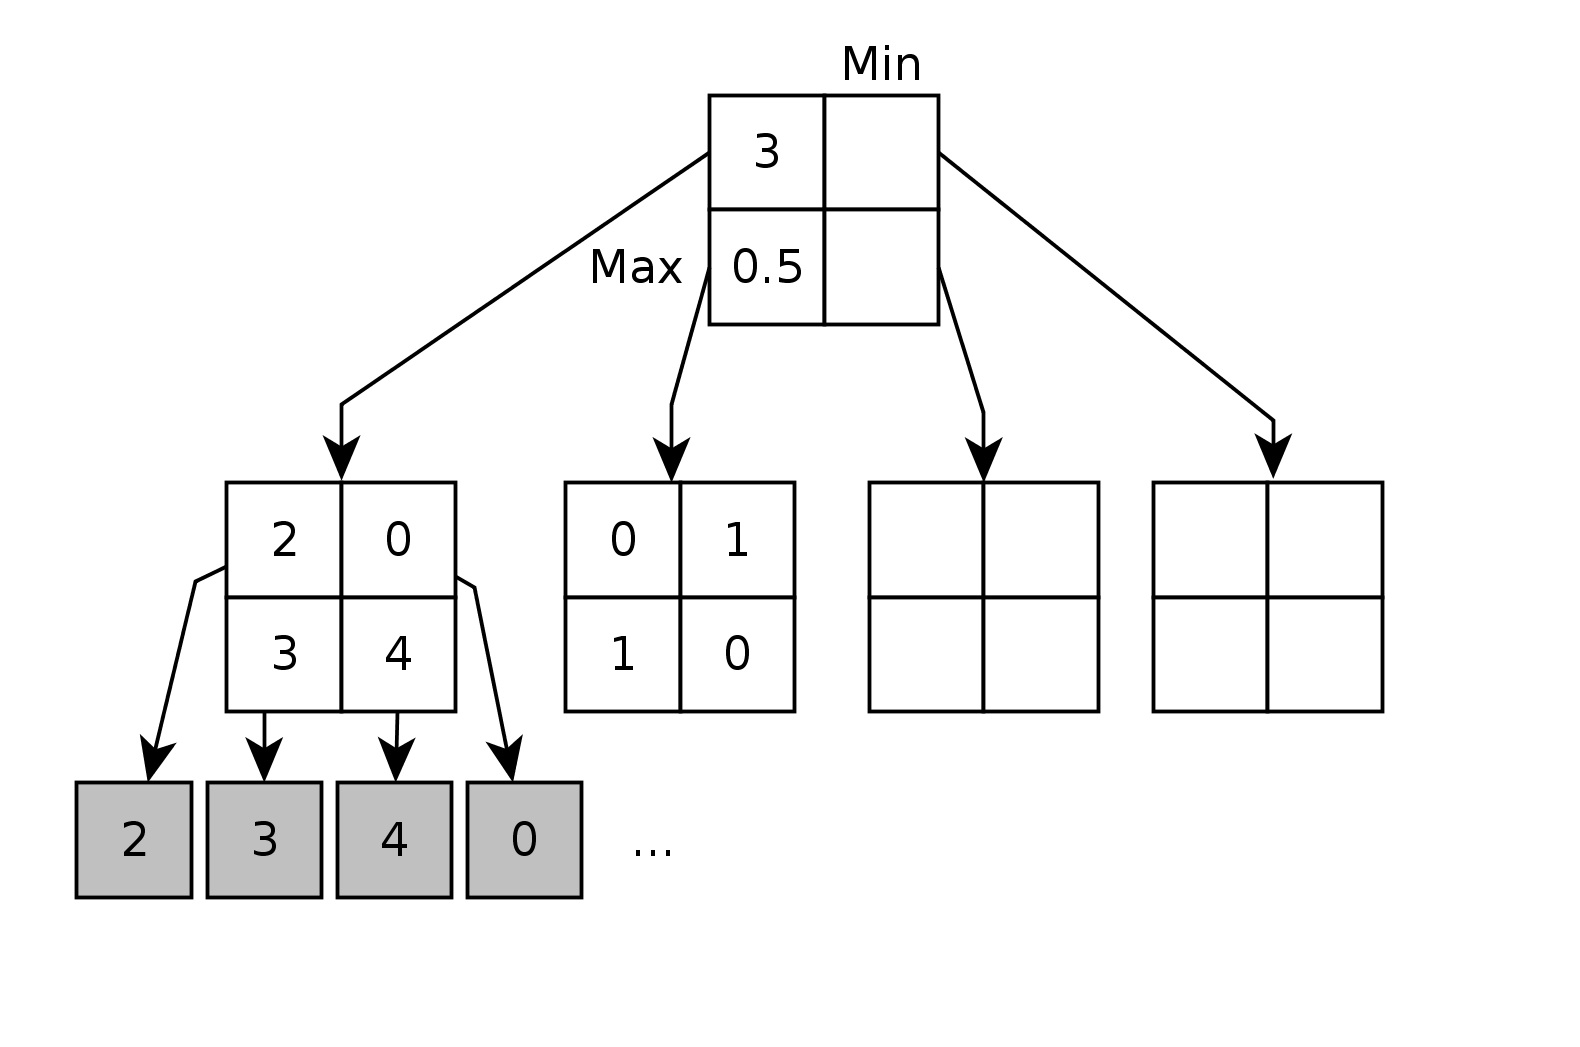
\includegraphics[width=6.0cm]{figures/tree} \hspace{0.03cm} 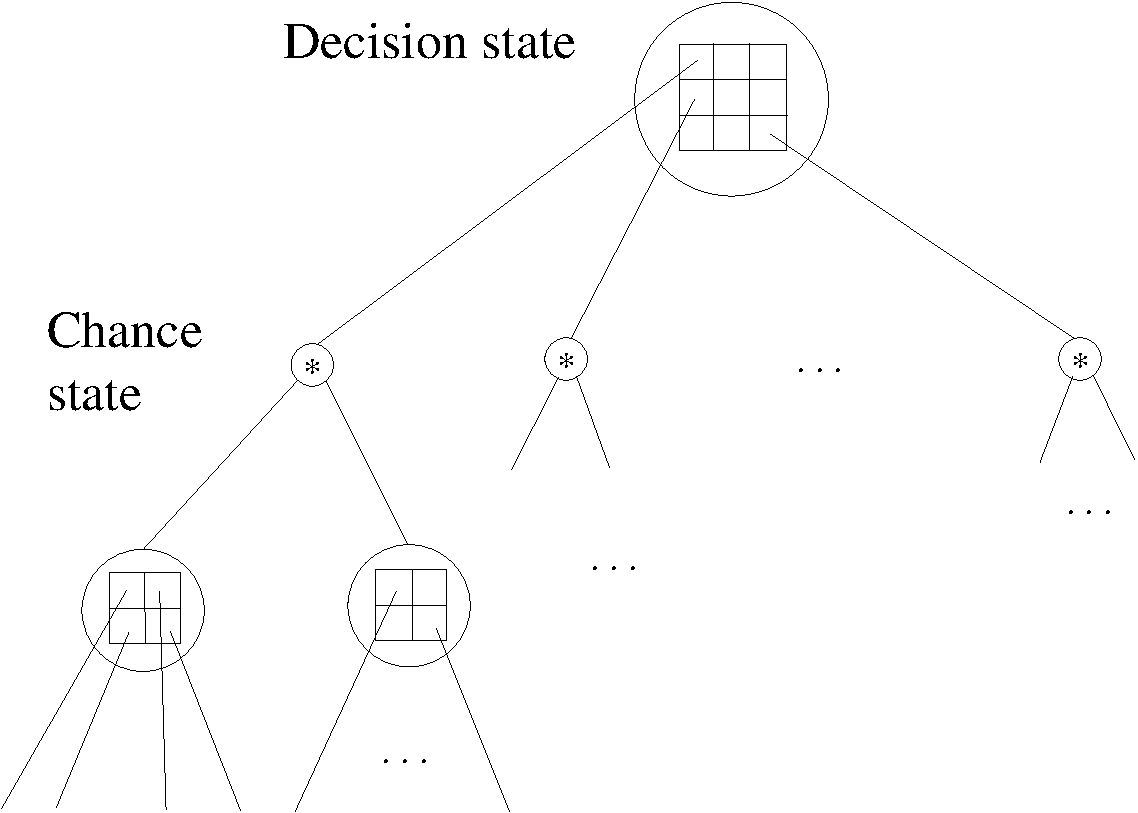
\includegraphics[width=5.5cm]{figures/goof3}\\
\end{subfigure}%\\
\caption{Examples of a two-player simultaneous game without chance nodes (left) which has Matching Pennies as a 
subgame, and a portion of 3-card Goofspiel including chance nodes (right).
The dark squares are terminal states. The values shown are optimal values that could be obtained by backward induction.\\
\label{fig:example}}
\end{figure}

A {\it matrix game} is a single step simultaneous move game with action sets $\cA_1$ and $\cA_2$. 
Each entry in the matrix $A_{rc}$ where $(r,c) \in A_1 \times A_2$ corresponds to a payoff (to player 1) if row $r$ is 
chosen by player 1 and column $c$ by player 2. 
For example, in Matching Pennies, each player has two actions (heads or tails). The row player receives a payoff of 1 
if both players choose the same action and 0 if they do not match. 
Two-player simultaneous move games are sometimes called {\it stacked matrix games} because at every state 
$s$ there is a joint action set $\cA_1(s) \times \cA_2(s)$ that either leads to a terminal state or (possibly after a 
chance transition) to a subgame which is itself another stacked matrix game. 

A {\it behavioral strategy} for player $i$ is a mapping from states $s \in \cS$
to a probability distribution over the actions $\cA_i(s)$, denoted $\sigma_i(s)$. 
Given a profile $\sigma = (\sigma_1, \sigma_2)$, define the probability of reaching a terminal state $z$ under $\sigma$ as 
$\pi^\sigma(z) = \pi_1(z) \pi_2(z) \pi_c(z)$, where each $\pi_i(z)$ is a product of probabilities of the actions taken 
by player $i$ along the path to $z$ ($c$ being chance's probabilities). Define $\Sigma_i$ to be the set of behavioral 
strategies for player $i$. A Nash equilibrium profile in this case is a pair of behavioral strategies optimizing
\begin{equation}\label{eq:ne}
V^* = \max_{\sigma_1 \in \Sigma_1} \min_{\sigma_2 \in \Sigma_2} \bE_{z \sim \sigma}[u_1(z)]
   = \max_{\sigma_1 \in \Sigma_1} \min_{\sigma_2 \in \Sigma_2} \sum_{z \in Z} \pi^\sigma(z) u_1(z).
\end{equation}
In other words, none of the players can improve their utility by deviating unilaterally. 
For example, the Matching Pennies matrix game has a single state and the only equilibrium strategy is to mix equally between 
both actions, \ie play with a {\it mixed strategy} (distribution) of $(0.5, 0.5)$ giving an expected payoff of $V^* = 0.5$. 
If the strategies also optimize Equation \ref{eq:ne} in each subgame starting in an arbitrary state, the equilibrium strategy 
is termed subgame perfect.

In two-player constant sum games a (subgame perfect) Nash equilibrium strategy is often considered to be optimal. It guarantees 
the payoff of at least $V^*$ against any opponent. Any non-equilibrium strategy has its nemesis, which will make it win less 
than $V^*$ in expectation. Moreover, subgame perfect NE strategy can earn more than $V^*$ against weak opponents. After the 
opponent makes a sub-optimal move, the strategy will never allow it to gain the loss back.
The value $V^*$ is known as the minimax-optimal value of the game
and is the same for every equilibrium profile by von Neumann's minimax theorem.

A two-player simultaneous move game is a specific type of two-player imperfect information extensive-form game. 
In imperfect information games, states are grouped into {\it information sets}: two states $s, s' \in I$ if the player 
to act at $I$ cannot distinguish which of these states the game is currently in. Any simultaneous move game can be modeled 
using an information set to represent a half-completed transition, \ie $\cT(s, a_1, ?)$ or $\cT(s, ?, a_2)$. 

The model described above is similar to a two-player finite horizon Markov Game~\cite{Littman94markovgames} with chance 
events. Examples of such games are depicted in Figure~\ref{fig:example}. 

\section{Offline Strategy Computation}

\subsection{Classical Backward Induction}

\section{Online Search}

\section{Empirical Evaluation}

\section{Conclusion}


\bibliographystyle{model1-num-names}
\bibliography{sm-journal}

%% Authors are advised to submit their bibtex database files. They are
%% requested to list a bibtex style file in the manuscript if they do
%% not want to use model1-num-names.bst.

%% References without bibTeX database:

% \begin{thebibliography}{00}

%% \bibitem must have the following form:
%%   \bibitem{key}...
%%

% \bibitem{}

% \end{thebibliography}


\end{document}

%%
%% End of file `elsarticle-template-1-num.tex'.
